\documentclass[tikz,border=10pt]{standalone}
\usepackage{tikz}
\begin{document}

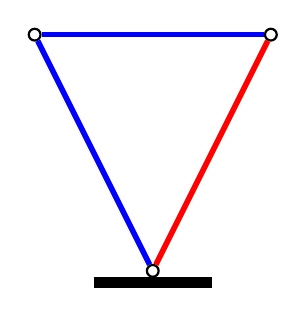
\begin{tikzpicture}[thick, scale=1.5]

% Nodes
\node[circle, draw, fill=white, inner sep=1.5pt] (A) at (0,2) {};
\node[circle, draw, fill=white, inner sep=1.5pt] (B) at (2,2) {};
\node[circle, draw, fill=white, inner sep=1.5pt] (C) at (1,0) {};

% Edges
\draw[blue, line width=2pt] (A) -- (B);
\draw[blue, line width=2pt] (A) -- (C);
\draw[red, line width=2pt] (B) -- (C);

% Ground
\draw[black, line width=4pt] (0.5,-0.1) -- (1.5,-0.1);

\end{tikzpicture}

\end{document}